\chapter{Rust概览}\label{ch02}
Rust给像本书一样的书籍的作者提出了一个挑战:赋予这门语言特色的并不是可以在第一页就展示出来的某些惊人的特性,而是如何设计这门语言来让它的各个部分可以无缝的协同工作,最终达到我们在上一章提到的目标:安全、高性能的系统级编程。这门语言的每一部分都在其他所有部分中得到了最好的证明。

因此,相比于一次着眼于一种语言特性,我们选择了几个简单但却完整的程序作为概览,每一个程序都会涉及到一些语言特性:

\begin{itemize}
    \item 作为热身,我们准备了一个简单的计算命令行参数的程序,以及相应的单元测试。这个程序展示了Rust的核心类型,并引入了\emph{trait}。
    \item 接下来,我们构建了一个web服务器。我们将会使用一个第三方库来处理HTTP的细节,并引入字符串处理、闭包、错误处理。
    \item 我们的第三个程序绘制了一个漂亮的图形,讲计算分布到多个线程来提高速度。这一部分包括一个泛型函数的示例,阐明了怎么处理类似于一个像素的概念,并展示了Rust对并发的支持。
    \item 最后,我们展示了一个使用正则表达式处理文件的健壮的命令行程序。这个程序展示了Rust标准库中处理文件的设施,和最常用的第三方正则表达式库。
\end{itemize}

Rust保证在对代码的性能影响最小的情况下防止未定义行为,这一保证影响了整个Rust中每个部分的设计,从标准的数据结构例如vector和string到Rust程序员使用第三方库的方式都受此影响。这些具体的细节书中都会提到,但是现在,我们想向你展示Rust是一门强大且有趣的语言。

当然,首先你要在你的计算机上安装Rust。

\section{rustup和Cargo}
安装Rust的最佳方式是使用\texttt{rustup}。访问\url{https://rustup.rs}并按照说明进行操作。

或者,你可以访问\href{https://www.rust-lang.org/}{Rust网站}来获取预构建好的Linux、macOS、Windows上的包。一些操作系统发行版里也包含Rust。我们推荐\texttt{rustup},因为它是专用于管理Rust安装的工具,就像Ruby的RVM和Node的NVM一样。例如,当一个新版本的Rust发布时,你只需要输入\texttt{rustup update}就可以完成更新。

在任何情况下,完成了安装之后,你应该可以通过命令行访问以下三条新命令:
\begin{minted}{text}
    $ cargo --version
    cargo 1.49.0 (d00d64df9 2020-12-05)
    $ rustc --version
    rustc 1.49.0 (e1884a8e3 2020-12-29)
    $ rustdoc --version
    rustdoc 1.49.0 (e1884a8e3 2020-12-29)
\end{minted}

这里,\texttt{\$}是命令提示符。在Windows上,可能是\texttt{C:\textbackslash>}或者别的类似的。这里我们运行了安装的三条命令,查询它们的版本。接下来让我们依次讲解每一个命令:
\begin{itemize}
    \item \texttt{cargo}是rust的编译管理器、包管理器和通用的工具。你可以使用Cargo来新建项目、构建并运行程序、管理所有代码中依赖的外部库。
    \item \texttt{rustc}是Rust的编译器。通常我们使用Cargo来调用编译器,但有时也需要直接运行它。
    \item \texttt{rustdoc}是Rust的文档工具。如果你在源代码中按照文档注释的格式写了文档,那么\texttt{rustdoc}可以通过它们构建出漂亮的HTML文档。和\texttt{rustc}一样,我们通常用Cargo来调用\texttt{rustdoc}。
\end{itemize}

方便起见,Cargo可以为我们创建新的Rust包,并设置好一些标准元数据:
\begin{minted}{text}
    $ cargo new hello
        Created binary (application) `hello` package
\end{minted}

这个命令创建了一个叫做\texttt{hello}的新的包目录,并准备好构建一个可执行程序。

进入包的顶级目录并查看:
\begin{minted}{text}
    $ cd hello
    $ ls -la
    total 24
    drwxrwxr-x.  4 jimb jimb 4096 Sep 22 21:09 .
    drwx------. 62 jimb jimb 4096 Sep 22 21:09 ..
    drwxrwxr-x.  6 jimb jimb 4096 Sep 22 21:09 .git
    -rw-rw-r--.  1 jimb jimb    7 Sep 22 21:09 .gitignore
    -rw-rw-r--.  1 jimb jimb   88 Sep 22 21:09 Cargo.toml
    drwxrwxr-x.  2 jimb jimb 4096 Sep 22 21:09 src
\end{minted}

我们可以看到Cargo创建了一个文件\texttt{Cargo.toml}来保存包的元数据。此时这个文件里还没有太多内容:
\begin{minted}{toml}
    [package]
    name = "hello"
    version = "0.1.0"
    authors = ["You <you@example.com>"]
    edition = "2018"

    # See more keys and their definitions at
    # https://doc.rust-lang.org/cargo/reference/manifest.html

    [dependencies]
\end{minted}

如果我们的程序中需要依赖的库,我们可以在这个文件中添加它们,Cargo将会负责下载、构建和更新这些库。我们将在\hyperref[ch08]{第8章}中详细讲述\texttt{Cargo.toml}文件。

Cargo已经为我们的包初始化好了\texttt{git}版本控制系统,创建了一个\texttt{.git}元数据目录和一个\texttt{.gitignore}文件。你可以通过向\texttt{cargo new}命令传递\texttt{--vcs none}参数来跳过这一步。

\texttt{src}子目录包含了实际的Rust代码:
\begin{minted}{text}
    $ cd src
    $ ls -l
    total 4
    -rw-rw-r--.  1 jimb jimb 45 Sep 22 21:09 main.rs
\end{minted}

看起来Cargo好像已经替我们写好了程序。\texttt{main.rs}中包含以下文本:
\begin{minted}{Rust}
    fn main() {
        println!("Hello, world!");
    }
\end{minted}

在Rust中,你甚至不需要编写自己的“Hello, World!”程序,这是新的Rust程序的模板:两个文件,总共13行。

我们可以从包中的任何目录调用\texttt{cargo run}命令来构建并运行我们的程序:
\begin{minted}{text}
    $ cargo run
        Compiling hello v0.1.0 (/home/jimb/rust/hello)
        Finished dev [unoptimized + debuginfo] target(s) in 0.28s
        Running `/home/jimb/rust/hello/target/debug/hello`
    Hello, world!
\end{minted}

这里,Cargo调用了Rust的编译器\texttt{rustc},然后运行了它生成的可执行文件。Cargo把可执行文件放在了顶层目录的\texttt{target}子目录下:
\begin{minted}{text}
    $ ls -l ../target/debug
    total 580
    drwxrwxr-x. 2 jimb jimb   4096 Sep 22 21:37 build
    drwxrwxr-x. 2 jimb jimb   4096 Sep 22 21:37 deps
    drwxrwxr-x. 2 jimb jimb   4096 Sep 22 21:37 examples
    -rwxrwxr-x. 1 jimb jimb 576632 Sep 22 21:37 hello
    -rw-rw-r--. 1 jimb jimb    198 Sep 22 21:37 hello.d
    drwxrwxr-x. 2 jimb jimb     68 Sep 22 21:37 incremental
    $ ../target/debug/hello
    Hello, world!
\end{minted}

如果需要的话,Cargo可以为我们清理生成的文件:
\begin{minted}{text}
    $ cargo clean
    $ ../target/debug/hello
    bash: ../target/debug/hello: No such file or directory
\end{minted}

\section{Rust函数}
Rust的语法借鉴自其他语言。如果你熟悉C、C++、Java或者JavaScript,你可以很快找到自己的方式来理解Rust的程序结构。这里有一个使用\href{https://en.wikipedia.org/wiki/Euclidean_algorithm}{欧几里得算法}计算两个整数的最大公约数的函数。你可以把它添加到\texttt{src/main.rs}的最后:
\begin{minted}{Rust}
    fn gcd(mut n: u64, mut m: u64) -> u64 {
        assert!(n != 0 && m != 0);
        while m != 0 {
            if m < n {
                let t = m;
                m = n;
                n = t;
            }
            m = m % n;
        }
        n
    }
\end{minted}

\texttt{fn}关键字(读作“fun”)创建了一个函数。这里,我们定义了一个叫\texttt{gcd}的函数,它有两个参数\texttt{m}和\texttt{n},类型都是\texttt{u64},也就是64位无符号整数。\texttt{->}词元指明了返回值类型:我们的函数返回一个\texttt{u64}类型的值。四个空格缩进是Rust的标准风格。

Rust的整数类型的名字代表了它们的大小和符号性:\texttt{i32}是有符号32位整数;\texttt{u8}是无符号8位整数(用于“字节”值)等等。\texttt{isize}和\texttt{usize}类型分别代表可以存下一个指针的有符号和无符号整数,在32位平台上它们就是32位,在64位平台上就是64位。Rust还有两种浮点数类型:\texttt{f32}和\texttt{f64},分别是IEEE标准的单精度和双精度浮点数类型,类似于C和C++中的\texttt{float}和\texttt{double}。

默认情况下,当变量初始化后,它的值就不能再被改变,但通过在参数\texttt{m}和\texttt{n}前加上\texttt{mut}关键字(读作“mute”,\emph{mutable}的缩写)就可以在函数体中对它们进行赋值。在实践中,大多数变量都不会被重新赋值,在阅读代码时\texttt{mut}关键字将是一个有用的提示。

函数体中首先调用了\texttt{assert!}宏,确保两个参数都不是0。\texttt{!}字符标志着这是宏调用,而不是函数调用。类似于C和C++中的\texttt{assert}宏,Rust中的\texttt{assert!}宏也会检查参数是否为真,如果不为真则中断程序,并输出一条有用的信息,其中包括断言失败的源码位置。这种终止的方式被称为\emph{panic}。和C和C++中断言可以被跳过不同,Rust总是检查断言,不管程序怎么编译。还有一个\texttt{debug\_assert!}宏,当程序被编译为release模式时会被跳过。

我们函数的主体是一个包含一条\texttt{if}语句和一条赋值语句的\texttt{while}循环。和C和C++不同,Rust的条件表达式不需要括号,但紧随其后的控制流语句需要花括号。

\texttt{let}语句声明了一个局部变量,比如函数中的\texttt{t}。我们不需要写出\texttt{t}的类型,因为Rust可以通过使用这个值的方式来推断它的类型。在我们的函数中,\texttt{t}只有和\texttt{m}、\texttt{n}相匹配,是\texttt{u64}类型时才可以正常运行。Rust只在函数体内推断类型:你必须写出函数参数和返回值的类型,就像我们所做的那样。如果你想指明\texttt{t}的类型,你可以写:
\begin{minted}{Rust}
    let t: u64 = m;
\end{minted}

Rsut有\texttt{return}语句,但是\texttt{gcd}函数并不需要。如果一个函数体以一个\emph{没有}分号结尾的表达式结尾,那么这个表达式的值就是函数的返回值。事实上,任何一个花括号包围的语法块都可以作为一个表达式。例如,这里有一个表达式打印出一条消息,然后返回\texttt{x.cos()}作为它的值:
\begin{minted}{Rust}
    {
        println!("evaluating cos x");
        x.cos()
    }
\end{minted}

在Rust中当控制流到达函数底部时利用这种形式返回值是一种很典型的做法,只有当在函数的中途显式地返回时才会使用\texttt{return}语句。

\section{编写并运行单元测试}
Rust语言内建有对测试的支持。为了测试我们的\texttt{gcd}函数,我们可以在\texttt{src/main.rs}的最后添加下列代码:
\begin{minted}{Rust}
    #[test]
    fn test_gcd() {
        assert_eq!(gcd(14, 15), 1);

        assert_eq!(gcd(2 * 3 * 5 * 11 * 17,
                       3 * 7 * 11 * 13 * 19),
                   3 * 11);
    }
\end{minted}

这里我们定义了一个叫\texttt{test\_gcd}的函数,它调用了\texttt{gcd}函数并检查返回值是否正确。喊函数上方的\texttt{\#[test]}标记\texttt{test\_gcd}是一个测试函数,这种函数在正常编译时会被跳过,但在使用\texttt{cargo test}命令时会被编译并自动调用。我们可以在整个源码树的任何位置定义测试函数,\texttt{cargo test}会自动收集它们并运行。

\texttt{\#[test]}标记是\emph{属性}的是一个示例。属性是一种为函数和其他声明标记额外信息的开放式系统,类似于C++和C\#中的属性,或者Java中的注解。它们被用来控制编译器警告和代码风格检查、条件编译(类似于C和C++中的\texttt{\#ifdef})、告诉Rust怎么和其它语言编写的代码交互等。随着继续深入我们将会看到更多使用属性的例子。

把\texttt{gcd}和\texttt{test\_gcd}函数的定义添加到\texttt{hello}包里之后,我们可以在包内的某个目录下按照如下方式运行测试:
\begin{minted}{text}
    $ cargo test
        Compiling hello v0.1.0 (/home/jimb/rust/hello)
         Finished test [unoptimized + debuginfo] target(s) in 0.35s
          Running /home/jimb/rust/hello/target/debug/deps/hello-2375a82d9e9673d7

    running 1 test
    test test_gcd ... ok
    
    test result: ok. 1 passed; 0 failed; 0 ignored; 0 measured; 0 filtered out
\end{minted}

\section{处理命令行参数}
为了让我们的函数能获取一些作为命令行参数传入的数字并打印出他们的最大公约数,我们可以把\texttt{src/main.rs}中\texttt{main}函数的代码替换为如下内容:
\begin{minted}{Rust}
    use std::str::FromStr;
    use std::env;

    fn main() {
        let mut numbers = Vec::new();

        for arg in env::args().skip(1) {
            numbers.push(u64::from_str(&arg)
                         .expect("error parsing argument"));
        }

        if numbers.len() == 0 {
            eprintln!("Usage: gcd NUMBER ...");
            std::process::exit(1);
        }

        let mut d = numbers[0];
        for m in &numbers[1..] {
            d = gcd(d, *m);
        }

        println!("The greatest common divisor of {:?} is {}",   numbers, d);
    }
\end{minted}

这是一个很大的代码块,让我们一步步来理解它:
\begin{minted}{Rust}
    use std::str::FromStr;
    use std::env;
\end{minted}

第一个\texttt{use}声明引入了标准库中的\texttt{FromStr} \emph{trait}。一个\texttt{trait}就是一些可以被实现的方法的集合。任何实现了\texttt{FromStr} trait的类型都有一个\texttt{from\_str}方法,这个方法尝试把一个字符串解析为该类型。\texttt{u64}类型实现了\texttt{FromStr},因此我们将调用\texttt{u64::from\_str}来解析命令行参数。尽管我们在程序中并没有使用到\texttt{FromStr}这个名字,但为了使用这个trait的方法,必须将它引入作用域。我们将会在第\hyperref[ch11]{第11章}讲解trait。

第二个\texttt{use}声明引入了\texttt{std::env}模块,它提供了一些和运行环境进行交互的函数和类型,包括\texttt{args}函数,它可以让我们获取到程序的命令行参数。

接下来移步到程序的\texttt{main}函数:
\begin{minted}{Rust}
    fn main() {
\end{minted}

我们的\texttt{main}函数不返回值,因此我们可以省略\texttt{->}和返回类型。

\begin{minted}{Rust}
    let mut numbers = Vec::new();
\end{minted}

我们声明了一个可变的局部变量\texttt{numbers},并将它初始化为一个空的向量。\texttt{Vec}是Rust的可变长的向量类型,类似于C++的\texttt{std::vector}、Python的\texttt{list}、或者JavaScript的\texttt{array}。即使vector被设计为动态伸缩,我们仍然需要将变量标记为\texttt{mut},这样Rust才允许我们向它的末尾添加元素。

\texttt{numbers}的类型是\texttt{Vec<u64>},一个\texttt{u64}的vector,但和之前一样,我们不需要写出类型。Rust将会为我们推断出它的类型,在这里我们把\texttt{u64}类型的值添加到了vector里,而且我们之后还把这个vector的元素传给了\texttt{gcd}函数,\texttt{gcd}函数的参数只能是\texttt{u64}。

\begin{minted}{Rust}
    for arg in env::args().skip(1) {
\end{minted}

这里我们使用了一个\texttt{for}循环来处理命令行参数,将每个参数命名为\texttt{arg}变量,然后执行循环体。

\texttt{std::env}模块的\texttt{args}函数返回一个\emph{迭代器},迭代器可以惰性产生每一个值,并指示我们何时迭代结束。迭代器在\texttt{Rust}中无处不在,标准库中还包含其他的迭代器例如产生vector中的每个元素、产生文件的每一行、产生通道收到的每一条消息、以及其他几乎所有可以循环处理的东西。Rust的迭代器非常高效:编译器通常能将它们翻译为和手写循环一样的代码。我们将会在\hyperref[ch15]{第15章}介绍该怎么使用它并给出一些示例。

除了和\texttt{for}循环一起使用之外,迭代器还有很多可以直接使用的方法。例如,\texttt{args}方法返回的迭代器的第一个值总是正在运行的程序名。我们想要跳过它,因此我们调用了迭代器的\texttt{skip}方法来生成一个省略了第一个值的新迭代器。

\begin{minted}{Rust}
    numbers.push(u64.from_str(&arg)
                 .expect("error parsing argument"));
\end{minted}

这里我们调用了\texttt{u64::from\_str}来尝试将命令行参数解析为64位整数。和通过\texttt{u64}类型的值调用的方法不同,\texttt{u64::from\_str}是一个和\texttt{u64}类型的值关联的方法,类似于C++和Java中的静态方法。\texttt{from\_str}函数不直接返回一个\texttt{u64}类型的值,而是返回一个\texttt{Result}类型的值来表示解析是否成功。一个\texttt{Rusult}类型的值有两种可能:

\begin{itemize}
    \item 一个写作\texttt{Ok(v)},表示解析成功,\texttt{v}就是解析出的值。
    \item 另一个写作\texttt{Err(e)},表示解析失败,\texttt{e}是解释失败的原因。
\end{itemize}

任何可能会失败的函数,例如输入输出或其他和操作系统交互的函数,都会返回\texttt{Result}值,\texttt{Ok}时会携带成功的结果——读写的字节数、打开的文件等等——\texttt{Err}时会携带错误码来指示错误的原因。和大多数现代编程语言不同,Rust没有异常:所有的错误都通过\texttt{Rust}或者panic来处理,这会在\hyperref[ch07]{第7章}中介绍。

我们使用Rust的\texttt{expect}方法来检查解析是否成功。如果结果是\texttt{Err(e)},\texttt{expect}会打印出包含\texttt{e}的描述错误的消息。如果结果是\texttt{Ok(v)},\texttt{expect}会简单的返回\texttt{v},之后我们才能把它添加到vector的尾部。

\begin{minted}{Rust}
    if numbers.len() == 0 {
        eprintln!("Usage: gcd NUMBER ...");
        std::process::exit(1);
    }
\end{minted}

空的数字集合没有最大公约数,因此我们检查vector是否不为空,如果为空就退出程序。我们使用\texttt{eprintln!}宏来把错误信息写入到标准错误输出流。

\begin{minted}{Rust}
    let mut d = numbers[0];
    for m in &numbers[1..] {
        d = gcd(d, *m);
    }
\end{minted}

这一个循环使用了变量\texttt{d},将它更新为目前的最大公约数。和之前一样,我们将\texttt{d}标记为可变的,因此我们在循环里给它赋值。

这个\texttt{for}循环有两个特别的地方。一个是\texttt{for m in \&numbers[1..];},操作符\texttt{\&}是什么意思?另一个是\texttt{gcd(d, *m);},\texttt{*m}里的\texttt{*}又是什么意思?事实上这两个细节是互补的。

到目前为止,我们的代码只操作过像整数这类固定内存大小的值。但是现在我们要迭代一个vector,它的值可能是任意大小——有可能非常大。在处理这类值时Rust是很谨慎的:它想让程序员自己控制对内存的消耗、明确每个值的生命周期,同时确保当内存不再被需要时立即释放内存。

因此当我们在迭代时,我们想告诉Rust这个vector的\emph{所有权}仍然属于\texttt{numbers},我们只是\emph{借用}它的值来进行循环。\texttt{\&numbers[1..]}中的\texttt{\&}运算符借用了vector中从第二个元素开始到最后一个元素的引用。\texttt{for}循环迭代引用的那些元素,每次迭代中用\texttt{m}借用每一个元素。\texttt{*m}中的\texttt{*}运算符\emph{解引用}了\texttt{m},返回了它所指向的值,也就是我们传递给\texttt{gcd}的第二个值。最后,因为\texttt{numbers}拥有vector的所有权,当\texttt{numbers}离开\texttt{main}的作用域时Rust会自动释放它的内存。

Rust对所有权和引用的规则时Rust的内存管理和安全并发的关键。我们将在\hyperref[ch04]{第4章}讨论他们,并在\hyperref[ch05]{第5章}讨论他们的伙伴。

要想舒服的使用Rust,你必须习惯这些规则,但在这篇概览中,你只需要知道\texttt{\&x}是借用\texttt{x}的引用,\texttt{*r}返回引用\texttt{r}指向的值。

继续我们的程序:
\begin{minted}{Rust}
    println!("The greatest common divisor of {:?} is {}", numbers, d);
\end{minted}

迭代完\texttt{numbers}的元素之后,程序把结果打印到标准输出流。\texttt{println!}宏接收一个模板字符串,用剩余参数替换掉模板字符串里的\texttt{\{...\}},并把结果写入到标准输出流。

与C和C++中的\texttt{main}函数成功执行结束时要返回0、执行失败时返回非0不同,Rust假设不管\texttt{main}返回什么值都代表成功执行结束。只有当显式调用\texttt{expect}或\texttt{std::process::exit}之类的才会导致程序以错误的状态码终止。

\texttt{cargo run}命令允许我们向程序传递参数,因此我们可以测试我们的命令行程序:
\begin{minted}{text}
    $ cargo run 42 56
       Compiling hello v0.1.0 (/home/jimb/rust/hello)
        Finished dev [unoptimized + debuginfo] target(s) in 0.22s
         Running `/home/jimb/rust/hello/target/debug/hello 42 56`
    The greatest common divisor of [42, 56] is 14
    $ cargo run 799459 28823 27347
        Finished dev [unoptimized + debuginfo] target(s) in 0.02s
         Running `/home/jimb/rust/hello/target/debug/hello 799459 28823 27347`
    The greatest common divisor of [799459, 28823, 27347] is 41
    $ cargo run 83
        Finished dev [unoptimized + debuginfo] target(s) in 0.02s
         Running `/home/jimb/rust/hello/target/debug/hello 83`
    The greatest common divisor of [83] is 83
    $ cargo run
        Finished dev [unoptimized + debuginfo] target(s) in 0.02s
         Running `/home/jimb/rust/hello/target/debug/hello`
    Usage: gcd NUMBER ...
\end{minted}

我们在这一节中用到了Rust标准库中的一小部分特性。如果你对其他的部分很好奇,我们强烈建议你去尝试Rust的在线文档。它的搜索功能很有用,甚至还包括到源代码的链接。当你安装Rust时\texttt{rustup}命令会自动在你的计算机上安装一份文档的拷贝。你可以在Rust的\href{https://www.rust-lang.org/learn}{网站}上查阅标准库的文档,或者通过如下命令在你的浏览器中查阅:
\begin{minted}{text}
    $ rustup doc --std
\end{minted}

\section{提供web页面}
Rust的一个强项就是发布在网站\href{https://crates.io}{crates.io}上的可以自由使用的包。\texttt{cargo}命令让你可以方便的使用crates.io的包:它将会按需下载正确的版本,构建并在需要时更新它。一个Rust包,无论是库还是可执行文件,都被称为一个\emph{crate}。Cargo和crates.io都是因为这个术语而得名。

为了展示它的工作方式,我们将会使用\texttt{actix-web}网络框架crate,\texttt{serde}序列化crate和其它它们依赖的crate来构建一个简单的web服务器。如\hyperref[f2-1]{图2-1}所示,我们的网站将会提示用户输入两个数字,然后计算它们的最大公约数。
\begin{figure}[htbp]
    \label{f2-1}
    \centering
    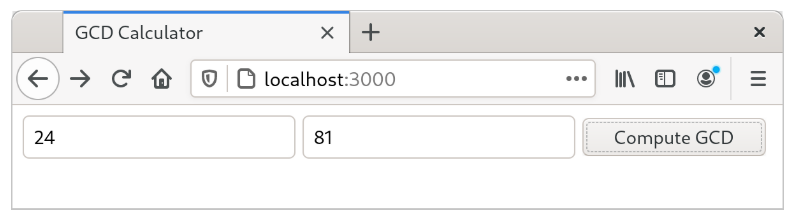
\includegraphics[width=0.8\textwidth]{../img/f2-1.png}
    \caption{提供计算最大公约数功能的web页面}
\end{figure}

首先,我们需要使用Cargo创建一个新的包,名称为\texttt{actix-gcd}:
\begin{minted}{text}
    $ cargo new actix-gcd
        Created binary (application) `actix-gcd' package
    $ cd actix-gcd
\end{minted}

然后,我们将编辑项目中的\texttt{Cargo.toml}文件来列举出我们需要的包,它的内容如下所示:
\begin{minted}{toml}
    [package]
    name = "actix-gcd"
    version = "0.1.0"
    authors = ["You <you@example.com>"]
    edition = "2018"

    # See more keys and their definitions at
    # https://doc.rust-lang.org/cargo/reference/manifest.html

    [dependencies]
    actix-web = "1.0.8"
    serde = { version = "1.0", features = ["derive"] }
\end{minted}

\texttt{Cargo.toml}中\texttt{dependencies}节的每一行都有一个cartes.io上的crate的名字和需要使用的版本。在这个例子中,我们需要\texttt{actix-web} crate的\texttt{1.0.8}版本和\texttt{serde} crate的\texttt{1.0}版本。crates.io上这两个crate可能还有更新的版本,但是通过指定我们测试成功的特定版本,可以保证即使这两个crate发布了新的版本,代码仍然可以正常工作。我们将会在\hyperref[ch08]{第8章}中详细的讨论版本管理。

crate有一些可选的特性:这些特性是有些用户可能用不到、但仍然需要包含在crate中的部分接口或实现。\texttt{serde}提供了一个非常简洁的方式来处理web表单中的数据,但是根据\texttt{serde}的文档,只有当我们选择了这个crate的\texttt{derive}特性,才可以使用这种方式,因此我们在\texttt{Cargo.toml}文件中制定了这个特性。

注意我们只需要指明那些我们直接使用的crate,\texttt{cargo}会自动下载它们依赖的其他crate。

在我们的第一个版本中,我们将保持web服务器的简洁:它将只提供一个页面,提示用户输入要计算的数字。将\texttt{actix-gcd/src/main.rs}中的内容替换为如下:
\begin{minted}{Rust}
    use actix_web::{web, App, HttpResponse, HttpServer};

    fn main() {
        let server = HttpServer::new( || {
            App::new()
                .route("/", web::get().to(get_index))
        });

        println!("Servering on http://localhost:3000...");
        server
            .bind("127.0.0.1:3000").expect("error binding server to     address")
            .run().expect("error running server");

    }

    fn get_index() -> HttpResponse {
        HttpResponse::Ok()
            .content_type("text/html")
            .body(
                r#"
                    <title>GCD Calculator</title>
                    <form action="/gcd" method="post">
                    <input type="text" name="n"/>
                    <input type="text" name="m"/>
                    <button type="submit">Compute GCD</button>
                    </form>
                "#
            )
    }
\end{minted}

我们以一条\texttt{use}声明开始,引入一些\texttt{actix-web}的定义。当我们写下\texttt{use actix\_web::\{...\}}时,花括号里的每一个名称都被导入到作用域中,这样我们就可以直接使用\texttt{HttpResponse},而不用每次都写出全名\texttt{actix\_web::HttpResponse}。(我们稍后才会使用\texttt{serde} crate)

我们的\texttt{main}函数很简单:它首先调用\texttt{HttpServer::new}来创建一个服务器,这个服务器会响应对\texttt{"/"}路径的get方法;然后打印出一条消息;最后让服务器监听本地机器上的3000 TCP端口。

我们传递给\texttt{HttpServer::new}的参数是Rust的\emph{闭包}表达式\texttt{|| \{ App::new() ... \}}。闭包是一种可以被当作函数来调用的值。这里定义的闭包没有参数,但如果需要参数的话,要写在\texttt{||}之间。\texttt{\{ ... \}}是闭包的函数体。当我们启动服务器时,Actix会启动一个线程池来处理到达的请求。每一个线程都会调用我们的闭包来获取一个\texttt{App}的拷贝,\texttt{App}的值将告诉它如何路由和处理请求。

